\subsubsection*{SOA参考架构}
\begin{figure}[H]
    \vspace{-0.5em}
	\centering
	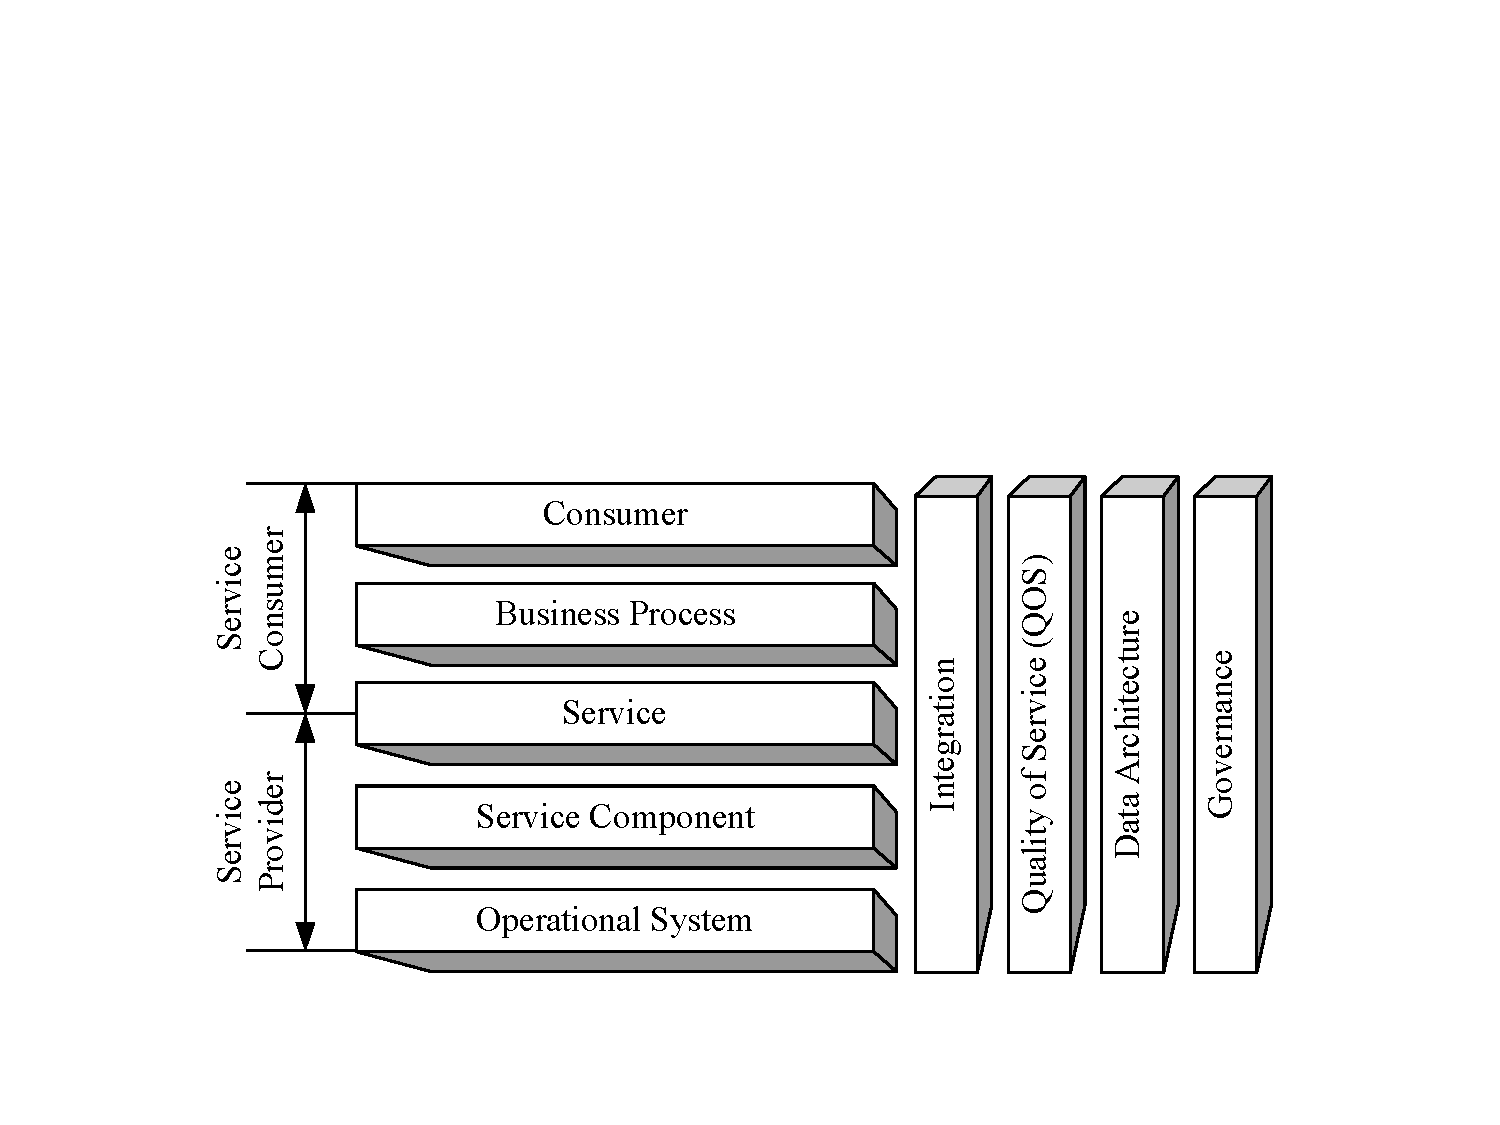
\includegraphics[width=0.7\textwidth]{SOA参考架构.pdf}
    \vspace{-1em}
\end{figure}

水平层:对功能性需求加以满足,五个水平层分为服务提供者和服务消费者两组:
\begin{itemize}
    \item 服务提供者(后台)
\end{itemize}
\begin{spacing}{1.2}
    \begin{table}[H]
    \centering
    \vspace{-0.5em}
    \begin{tabular}{|c|l|}
        \hline
        \textbf{操作型系统层} & \begin{tabular}[c]{@{}l@{}}包括ISV(独立软件开发商)提供的打包应用、客户应用、遗留系统等。\\ 该层的应用(不一定面向服务)往往只为一个目的、服务于一类特定用户。\end{tabular}                                                                                                                                         \\ \hline
        \textbf{服务组件层}  & \begin{tabular}[c]{@{}l@{}}包括用于提供用以实现服务层中所定义服务的代码容器,其中一个服务组件依赖于\\ 操作系统型层次中的一些打包组件、服务层中的一些服务、业务过程层中的一些业\\ 务过程。\\ 该层可能实现多个方法,但其中只有一部分会被服务层封装为服务。\\ 从调用角度出发,服务组件层负责完成输入转换和输出配置的自动化逻辑。\end{tabular}                                                       \\ \hline
        \textbf{服务层}    & \begin{tabular}[c]{@{}l@{}}将SOA三角操作模型扩展为综合的逻辑层次,以支持服务注册、服务分解、服务\\ 发现、服务绑定、接口聚合和生命周期管理。服务层负责定位合适的服务提供者,\\ 并绑定到具体目标服务接口;同时负责以服务组合的形式封装服务对外提供。\\ \textbf{服务簇}是服务层中的核心概念,是一类从概念上服务于同一业务功能的服务集合。\\ 服务簇中的服务可以由不同的功能提供者所发布,并在具体的特性上有所差异(但\\ 都能满足业务功能需求)。\end{tabular} \\ \hline
    \end{tabular}
\end{table}
    \vspace{-2.5em}
\end{spacing}

\begin{itemize}
    \item 服务消费者(前台)
\end{itemize}

\begin{spacing}{1.15}
    \begin{table}[H]
    \centering
    \begin{tabular}{|c|l|}
    \hline
    \textbf{服务层}   & 服务层作为前后台连通的接口,功能同上。   \\ \hline
    \textbf{业务过程层} & \begin{tabular}[c]{@{}l@{}}以组合和分解的方式来处理业务逻辑。\\ 从组合角度出发,业务过程层使用服务层来快速组合服务,并协调业务过程来满足消\\ 费者需求;从分解的角度出发,业务过程层将业务需求分解为能够由概念上的服务簇\\ 所表达的任务。\\ 业务服务层着眼于从协作和管理一些列过程的角度出发,采用也无流程来构建SOA\\解决方案。\\ 存在两种组合方式:编排和编导(二者功能上等价,主流模式为编排)。\end{tabular} \\ \hline
    \textbf{消费者层}  & \begin{tabular}[c]{@{}l@{}}消费者层负责表达对业务过程层、服务层及其他层次的调用。\\ 通过为业务服务快速构建用户接口来满足消费者的需求。\\ 消费者层负责构建SOA解决方案与用户之间进行交互的前端接口。\\ 消费者层可能需要同时支持不同种类的用户和渠道。\\ 为了提升展现性能,往往需要支持缓存机制。\end{tabular}                                                         \\ \hline
    \end{tabular}
\end{table}
    \vspace{-1em}
\end{spacing}

垂直层:对当前系统进行支撑以及实现服务质量、非功能性需求
\begin{spacing}{1.15}
        \begin{table}[H]
        \centering
        \resizebox{\textwidth}{!}{
        \begin{tabular}{|c|l|}
        \hline
        \textbf{集成层}                                                   & \begin{tabular}[c]{@{}l@{}}SOA解决方案中的关键支持部件,用以在服务请求者和服务提供者之间,完成服务请求的 \\ 中介、路由和转换。\end{tabular}                                                 \\ \hline
        \textbf{\begin{tabular}[c]{@{}c@{}}服务质量层\\ (QoS)\end{tabular}} & \begin{tabular}[c]{@{}l@{}}从各个方面(可用性、可靠性、安全性等非功能性需求)提供解决方案层级的QoS管理。\\ 服务质量层不关注于服务层级的QoS控制,而是着眼于为解决方案层级的 QoS 控制提供 \\ 支持、跟踪、监视和管理。\end{tabular} \\ \hline
        \textbf{数据架构层}                                                 & \begin{tabular}[c]{@{}l@{}}为了方便值链集成(集成来源于不同开发方的服务),数据架构层为领域相关的数据架构提 \\ 供统一的表达和支持机制。\end{tabular}                                             \\ \hline
        \textbf{治理层}                                                   & \begin{tabular}[c]{@{}l@{}}提供用以确保 SOA 解决方案的设计原则;通常使用最佳实践的方式,来提供如何在各个层 \\ 次中构建 SOA 解决方案的原则、如何监管运营中的系统,并在运行时处理异常的原则。\end{tabular}               \\ \hline
        \end{tabular}}
    \end{table}
    \vspace{-2em}
\end{spacing}

\begin{itemize}
    \item SOA-RA 展示了如何将 SOA 解决方案构建为一组逻辑层的抽象。
    \item SOA-RA 是一种松耦合的架构,因为每个层不严格隐藏在上面的层之中。
    \item SOA-RA 是一个企业级架构模板,通过定义参考架构指导在企业级别上创建 SOA 解决方案。
    应用 SOA-RA 模型来定义 SOA 导向的系统架构的一种实践称为服务导向建模和架构(SOMA)。
    \item 在SOA-RA层中配置组件定义了三个步骤:
    \vspace{-0.8em}
    \begin{multicols}{3}
    \begin{itemize}
        \item 服务识别步骤
        \item 服务规范步骤
        \item 服务实现步骤
    \end{itemize}
    \end{multicols}
    \vspace{-1em}
\end{itemize}